\documentclass[tikz]{standalone}
\usepackage{tkz-graph}
\usepackage{amsmath,amssymb}
\usepackage{xcolor}
\usetikzlibrary{calc}
\usetikzlibrary{positioning}

\begin{document}

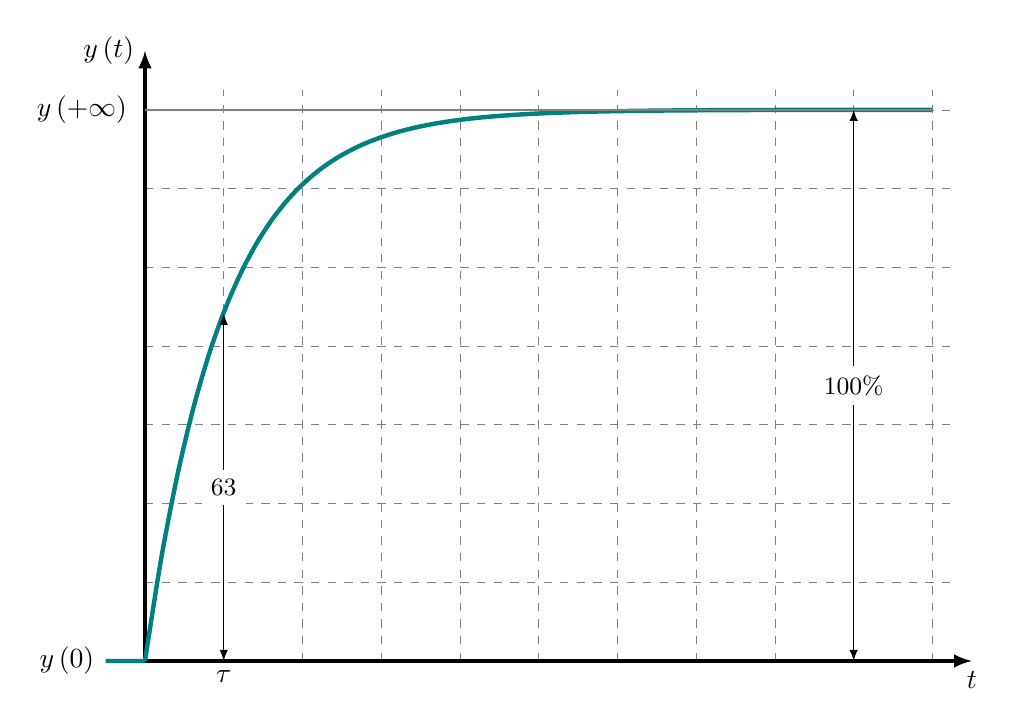
\begin{tikzpicture}
	\draw [help lines, dashed] (0,0) grid  (10.25,7.25);
	\draw [very thick, latex-latex] (0, 7.75) node[left] {\(y\left(t\right)\)} |-  (10.5,0) node[below] {\(t\)};
	\draw [ultra thick, teal]  (-0.5, 0) node[left,black](s0) {\(y\left(0\right)\)} --
	++(0.5, 0) plot[domain=0:10, samples=50, smooth]({\x}, {7*(1-exp(-\x))});


	\draw [thick, gray] (0,7) node[left=0.1cm, black] {\(y\left(+\infty\right)\)} -- (10, 7);
	\draw [latex-latex] (1, 0.63*7) -- (1,0) node[below]{\(\tau\)} node[midway, fill=white]{\small \(63\)};

	\draw [latex-latex] (9, 7) -- (9,0) node[midway, fill=white] {\small \(100\%\)};

\end{tikzpicture}

\end{document}

